% !TEX root = ../paper_zh.tex

\section{UAV-TAlign 参考框架}

\subsection{问题定义}

UAV-TAlign 用于实例化 UAV-TAlign-12K 的场景级评测轨道。对每个场景，输入是一组配对的无人机
RGB 与红外帧
$S = \{(I_i^R, I_i^T)\}_{i=1}^N$。视点变化、跨分辨率感知、热成像外观差异和光照变化会使
各帧估计具有异质的支撑质量。目标是恢复一个从红外到 RGB 的场景单应性，并刻画其运行置信度。

该定义把配准表述为多帧证据整合问题，而非单对图像选择问题。框架需要把质量不一的逐帧估计
转化为几何稳定且跨模态一致的场景变换。对于一个选定图像对，从红外到 RGB 的证据表示为作用于
齐次图像坐标的单应矩阵 $H_i \in \mathbb{R}^{3 \times 3}$：
\begin{equation}
\tilde{\mathbf{p}}^{R}_{ij} \sim H_i \tilde{\mathbf{p}}^{T}_{ij},
\qquad
H_i = \arg\min_H \sum_{j \in \mathcal{I}_i}
\rho\!\left(\left\|\pi(H\tilde{\mathbf{p}}^{T}_{ij}) -
\mathbf{p}^{R}_{ij}\right\|_2^2\right),
\label{eq:pairwise_homography_zh}
\end{equation}
其中，$\mathcal{I}_i$ 表示鲁棒估计得到的内点集合，$\pi(\cdot)$ 将齐次坐标转换为图像坐标，
$\rho(\cdot)$ 是鲁棒估计损失。场景级问题是在证据集合 $\{H_i\}$ 上估计共识变换
$\bar{H}_S$，并赋予其规范产品状态。

\begin{figure}[t]
\centering
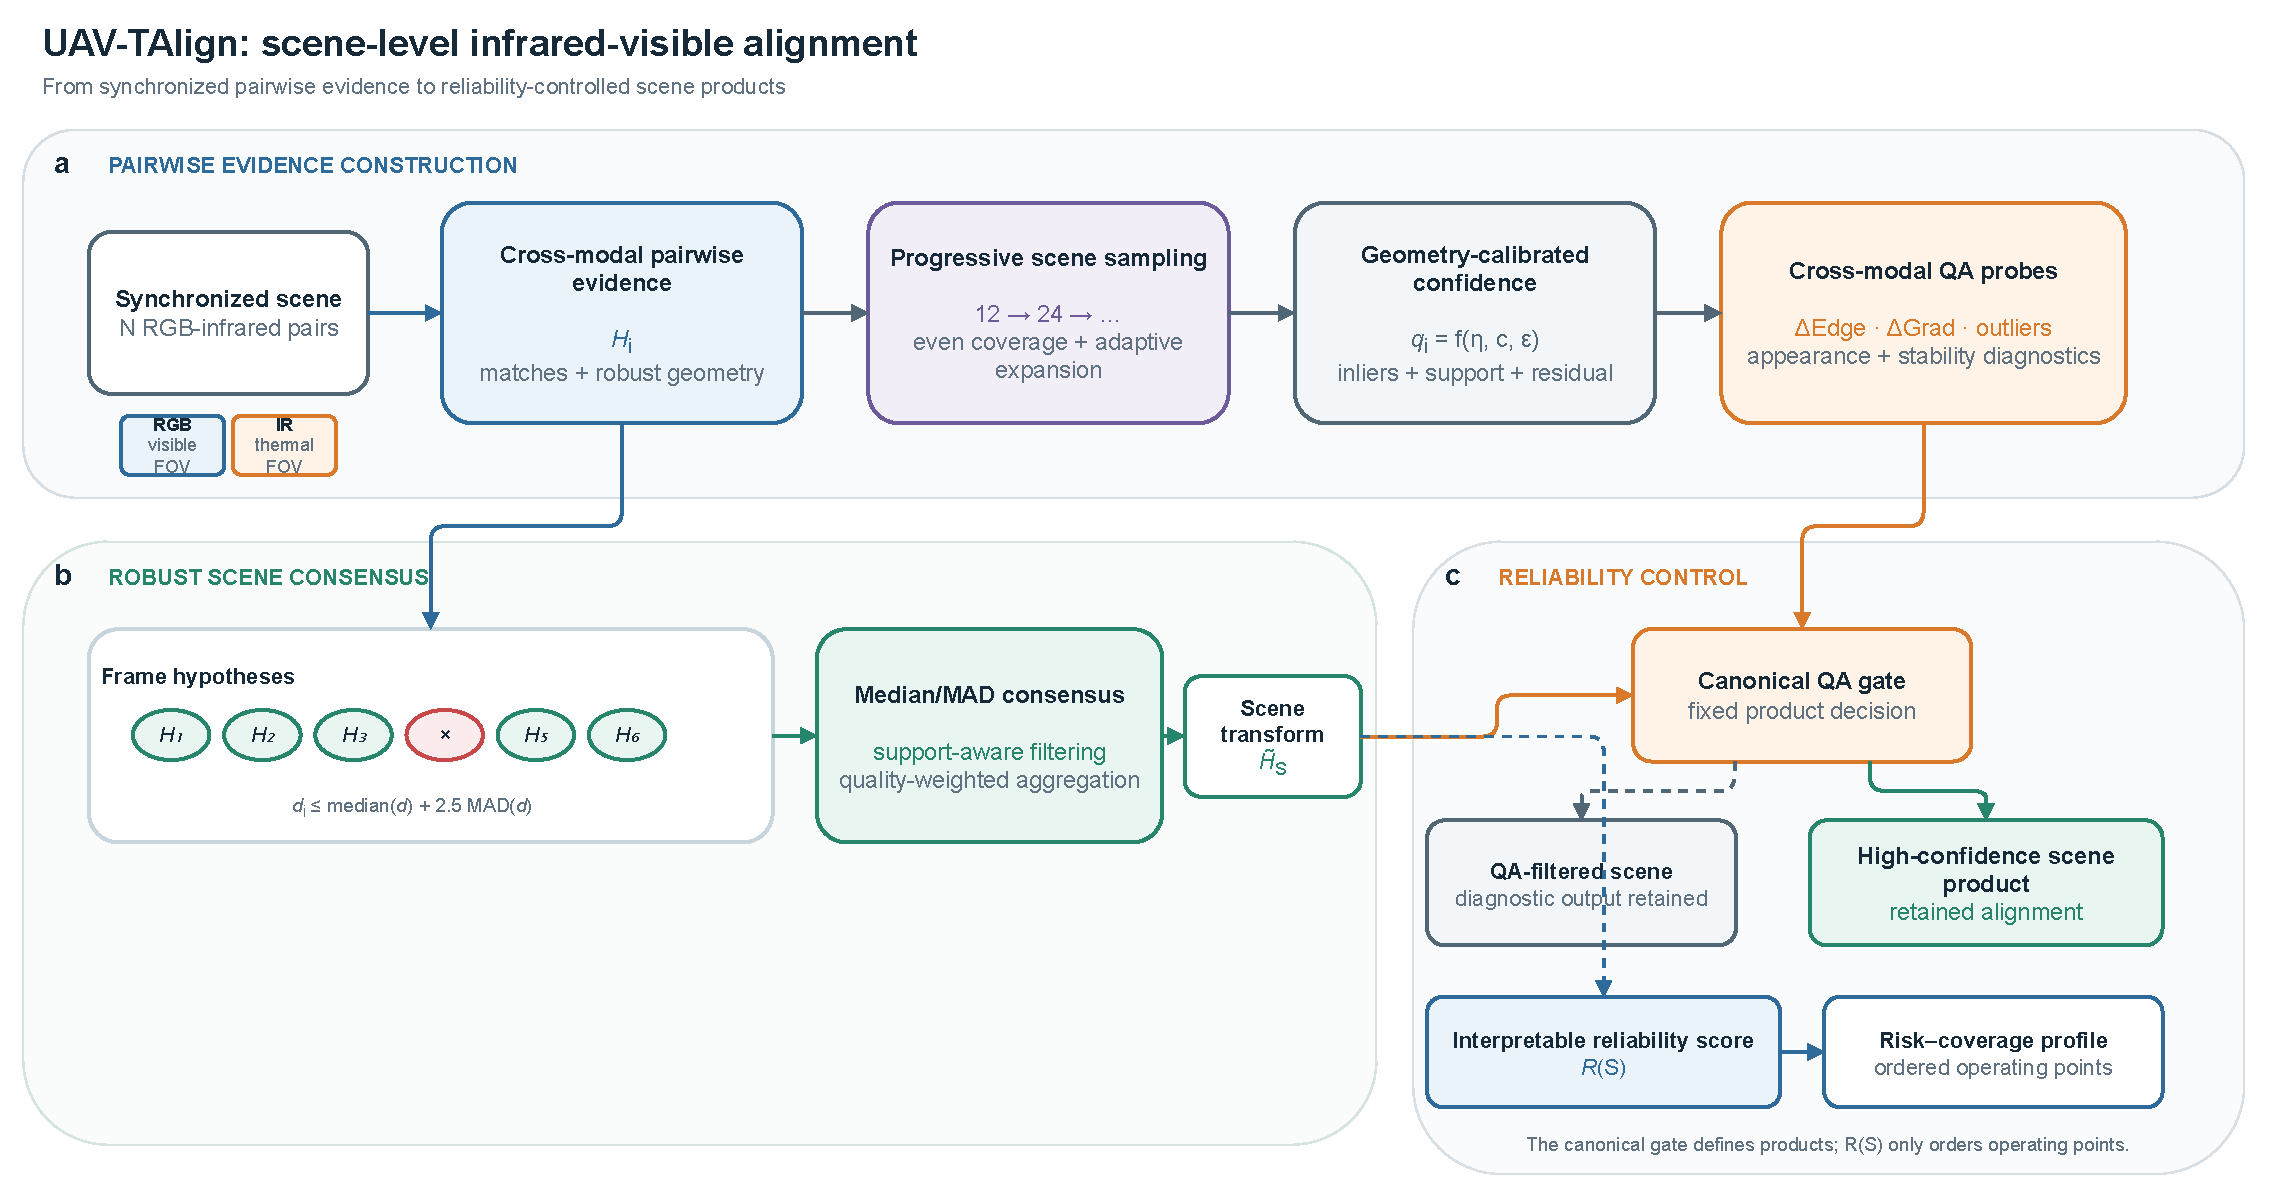
\includegraphics[width=\textwidth]{figures/fig03_scene_framework.pdf}
\caption{UAV-TAlign 场景级对齐框架。（a）同步 RGB-红外图像对依次经过成对单应性生成、渐进式证据
调度、几何校准帧可靠性、鲁棒中位数/MAD 共识和跨模态质量验证；（b）共识支撑外的逐帧假设在固定
规范门控之前被剔除，门控定义高置信产品，可解释分数则独立用于运行覆盖率排序。}
\label{fig:scene_framework_zh}
\end{figure}

\subsection{成对证据生成器}

UAV-TAlign 使用预训练多模态匹配器生成成对证据。参考实现采用 MINIMA 的 RoMa 分支，其余
阶段则可以接收任意兼容匹配器输出的单应性与几何诊断量
\cite{edstedt2024roma,ren2025minima}。

\subsection{渐进式证据调度}

UAV-TAlign 从一个紧凑、均匀分布的帧子集开始，并以确定性阶段逐步扩展支撑集合。调度规模随
场景长度变化，必要时可以覆盖完整序列。当接受支撑、共识稳定性和跨模态质量条件满足时停止扩展；
否则评测下一阶段子集。

在每个阶段内，均匀分布采样提供可复现的时间或索引覆盖。随机选择变体通过独立的多随机种子
敏感性分析进行评测。

\subsection{几何校准帧可靠性}

对于每个选定图像对，匹配器产生跨模态对应关系和逐帧单应性估计。UAV-TAlign 测量匹配数量、
内点支撑、内点率、重投影误差和空间覆盖率。当这些统计量满足几何质量准则时，对应帧进入场景
候选池。该处理遵循标准单应性估计与鲁棒拟合方法
\cite{hartley2004multiple,fischler1981ransac,barath2019magsac,barath2020magsacpp}。

每个接受帧还会获得一个连续质量权重。该权重综合内点率、空间覆盖率、重投影质量、匹配器置信度
以及内点支撑，使具有更强几何依据的单应性在场景聚合中具有更大影响。归一化帧质量权重写为：
\begin{equation}
q_i =
\alpha_r \phi(r_i) +
\alpha_c \phi(c_i) +
\alpha_e \phi(e_i) +
\alpha_m \phi(m_i) +
\alpha_n \phi(n_i),
\qquad
\sum_k \alpha_k = 1,\ \alpha_k \ge 0,
\label{eq:frame_quality_zh}
\end{equation}
其中，$r_i$ 是内点率，$c_i$ 是空间覆盖率，$e_i$ 是重投影质量，$m_i$ 是匹配器置信度，
$n_i$ 是内点支撑，$\phi(\cdot)$ 将各诊断量映射到一致的质量方向。所有 UAV-TAlign-12K
评测均使用固定权重。

\subsection{鲁棒场景共识}

在获得足够的逐帧单应性后，UAV-TAlign 构建鲁棒场景共识。首先将单应性映射到参数空间，以
中位数作为中心参考，并采用中位数绝对偏差（MAD）准则剔除不稳定估计；随后使用上述帧质量分数
对保留单应性进行加权聚合。令 $\mathbf{h}_i$ 表示 $H_i$ 的尺度归一化向量形式，则共识集合为：
\begin{equation}
\begin{aligned}
\mathbf{h}^{\mathrm{med}}_S
&= \operatorname{median}_{j \in \mathcal{A}_S}(\mathbf{h}_j), \\
d_i &= \left\|\mathbf{h}_i - \mathbf{h}^{\mathrm{med}}_S\right\|_2, \\
m_d &= \operatorname{median}_{j \in \mathcal{A}_S}(d_j), \\
s_d &= \operatorname{median}_{j \in \mathcal{A}_S}|d_j-m_d|, \\
\mathcal{C}_S &= \left\{i \in \mathcal{A}_S: d_i \le m_d + 2.5s_d\right\}.
\end{aligned}
\label{eq:consensus_set_zh}
\end{equation}
其中，$\mathcal{A}_S$ 是鲁棒共识前的接受帧集合。场景变换通过质量加权聚合得到：
\begin{equation}
\bar{\mathbf{h}}_S =
\frac{\sum_{i \in \mathcal{C}_S} q_i \mathbf{h}_i}
{\sum_{i \in \mathcal{C}_S} q_i},
\qquad
\bar{H}_S = \operatorname{mat}(\bar{\mathbf{h}}_S).
\label{eq:scene_consensus_zh}
\end{equation}

框架同时记录聚合变换周围的稳定性诊断，包括相对于聚合结果的单应性离散度，以及被鲁棒剔除的
逐帧估计比例。这些诊断量把共识形成过程与最终场景产品决策联系起来。

\subsection{跨模态场景验证}

最后阶段融合几何支撑与跨模态场景一致性。UAV-TAlign 在代表帧上测量优化后变换的边缘重叠增益、
梯度 NCC 增益、改善帧比例和严重相对离群点。同时记录接受帧支撑、平均内点率、平均重投影误差、
空间覆盖率、相对于聚合变换的离散度，以及鲁棒剔除比例。

规范决策采用基线感知验证规则。高置信产品需要同时具备较强的接受帧支撑、稳定的共识几何、
受控的基线相对离群点和改善后的梯度对齐。为绘制运行曲线，使用一个固定、可解释的可靠性分数
汇总同一组诊断量：
\begin{equation}
\begin{aligned}
R(S) ={}&
\beta_a A_S +
\beta_o (1-O_S) +
\beta_j (1-J_S) \\
&+
\beta_e \Delta E_S +
\beta_g \Delta G_S +
\beta_{\gamma} \Gamma_S,
\qquad
\sum_k \beta_k = 1 .
\end{aligned}
\label{eq:reliability_score_zh}
\end{equation}
其中，$A_S$ 是接受帧支撑，$O_S$ 是严重基线相对离群点比例，$J_S$ 是鲁棒共识剔除比例，
$\Delta E_S$ 与 $\Delta G_S$ 分别为边缘和梯度增益代理量，$\Gamma_S$ 汇总几何诊断量。
规范决策要求满足最低接受帧假设数量，并通过两条固定验证路径之一：
\begin{equation}
y_S =
\mathbb{1}\!\left[
N_S \ge N_{\min}
\right]
\mathbb{1}\!\left[L_S \lor W_S\right].
\label{eq:canonical_gate_zh}
\end{equation}
其中，$L_S$ 表示主要边缘/梯度路径，$W_S$ 表示联合接受支撑、共识几何、相对离群点控制和
梯度改善的高模态路径。$R(S)$ 用于可靠性--覆盖率分析中的场景排序，$y_S$ 则定义规范的高置信
对齐产品集合。

图~\ref{fig:consensus_qa_zh} 在一组匹配场景对照上揭示内部证据流：即使接受帧数量相同，引入共识
剔除与跨模态离群点后，仍可得到不同的场景产品决策。

\begin{figure}[t]
\centering
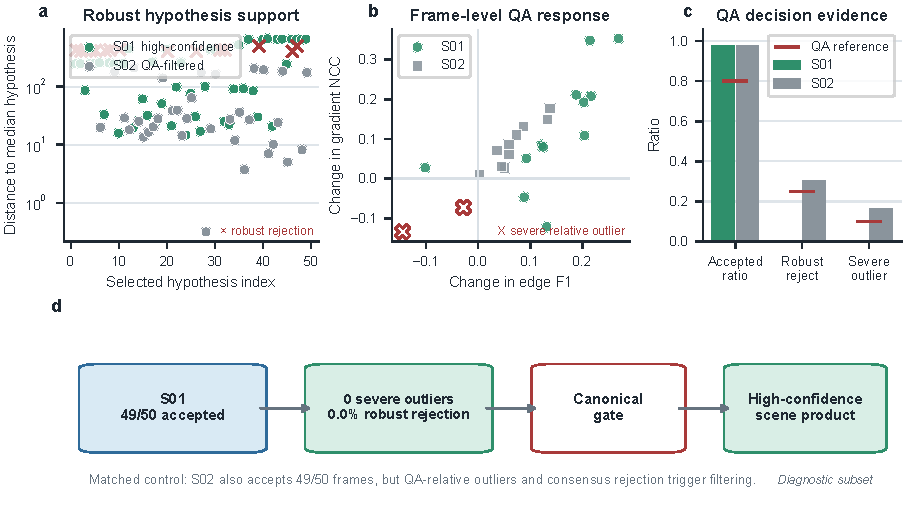
\includegraphics[width=\textwidth]{figures/fig04_consensus_qa.pdf}
\caption{匹配场景对照上的鲁棒共识与跨模态质量验证机制。（a）中位数/MAD 支撑簇确定聚合证据；
（b）逐帧边缘与梯度变化揭示严重相对离群点；（c）接受支撑、鲁棒剔除和离群点控制构成互补决策
证据；（d）固定规范门控将这些信号转换为高置信场景产品。}
\label{fig:consensus_qa_zh}
\end{figure}
